\chapter{Introduction}
\label{chapter:introduction}
\section{Nuclear matter under extreme conditions}
The quest for the matter and its properties under extreme highly density and temperature has fundamental importance.
Understanding nuclear matter and under these conditions help to understand questions from the early dynamics of the universe to the neutron star merger simulation for the gravitational wave studies.
It also help to enrich the understanding of the fundamental theory of the strong interaction and basics to the nuclear physics: the Quantum Chromodynamics (QCD).

\paragraph{Quantum Chromodynamics}
QCD describes the interaction of objects that carries ``color'' charges.
Quarks (fermions) and gluons (bosons) are its elementary degrees of freedom. 
The QCD Lagrangian (with one flavor of quark) is,
\begin{eqnarray}
\mathcal{L} = \bar{\psi_i} \left(i\gamma_\mu D^\mu_{ij} -m \delta_{ij} \right)\psi_j - \frac{1}{4}G_{\mu\nu}^a G^{\mu\nu,a},
\end{eqnarray}
where $\psi_i$ the Dirac spinor of the quark field with $i$ the color index.
\begin{eqnarray}
D_{ij}^\mu = \partial^\mu - i g T_{ij}^a A^{\mu, a}
\end{eqnarray}
is the covariant derivative, containing the interaction between quark field and the gluon field with coupling strength $g$.
Here $T_{ij}^a$ are the generators of the SU(3) group in the fundamental representation and the generators satisfies the commutation relation,
\begin{eqnarray}
[T^a, T^b] = i f^{abc} T^c
\end{eqnarray}
where $f^{abc}$ are known as the structure constants of SU(3).
The field tensor of gluon with color $a$ is,
\begin{eqnarray}
G^{\mu\nu,a} = \partial^\mu A^{\nu, a} - \partial^\nu A^{\mu, a} + g f^{abc} A^{\mu,b}A^{\mu,c}
\end{eqnarray}
The first term is the kinetic term, and the second term is the gluon field self-interation (also with strength $g$) is a unique feature of the non-Abelian gauge field.

\paragraph{Asymptotic freedom and confinement}
Due to quantum fluctuations, the effective coupling constant $g$ changes with the energy scale of a process. 
The rate of change of $g$ with respect to the scale parameter is called the $\beta$-function,
\begin{eqnarray}
\frac{\partial g}{\partial \ln\mu} = \beta(g),
\end{eqnarray}
which can be evaluated as a perturbation series of $g$.
At leading order, the QCD $\beta$ function with number of colors $N_c$ and $n_f$ flavors of fermion is,
\begin{eqnarray}
\beta(g) = - \left( \frac{11}{3}N_c - \frac{2}{3}n_f \right) \frac{g^3}{16\pi^2}.
\end{eqnarray}
This $\beta$ function is negative for QCD ($N_c=3$) using realistic numbers of quark flavors $n_f = 2\cdots 6$, meaning the effective coupling constant decreases with increasing energy scale.
The property is known as the asymptotic freedom of QCD because the interaction becomes small at asymptotically high energy, which also makes possible the use of perturbation theory at high energy.

Often a strong coupling constant is defined as $\alpha_s = g^2/4\pi$.
Using the leading order $\beta$-function, its scale dependence is
\begin{eqnarray}
    \alpha_s(Q^2) = \frac{4\pi}{\left(\frac{11}{3}N_c - \frac{2}{3}n_f\right)\ln\left(\frac{Q^2}{\Lambda^2}\right)}.
\end{eqnarray}
The integration constant has been absorbed into the QCD scale parameter $\Lambda$.
Therefore, at least in perturbation theory, $\Lambda$ becomes the only parameter of QCD. 
Its value is determined by anchoring $\alpha_s(\mu)$ to the experimental measurement at a fixed scale, for example, $\alpha_s(M_z) = 0.1185$ at the scale equal to the $Z$ boson mass.
The leading order $\Lambda$ is then around $200$ MeV.

The decreasing of $\alpha_s(Q)$ is logarithmic slow at high energy, but it rises quickly approaching with $Q$ approaching $\Lambda$ from above.
Even before reaching this scale, the coupling constant is already too large for a reliable perturbative calculation.
Near the $\Lambda$ scale, QCD enters the non-perturbative region,
and at this long distances only hadrons exists as colorless bound states of quarks and gluons.
The fact that colors not directly observed at large distances is knowns as ``color confinement'' of QCD. 
To pull a quark out of the hadron, the color field becomes so strong that eventually more quark-anti-quark pairs populated in-between the pulled quark and the remnant and forms new colorless hadrons.

Depending on its valance quarks (quarks that carry the net quantum number of the hadron) content, hadrons are generally categorized as baryons and mesons.
Baryon has three valance quarks or anti-quarks, such as neutrons and protons.
Meson has a valance quark and an anti-quark, such as pion and kaon.
Hadrons are also populated with sea-quarks and gluons that are constantly produced and annihilated as quantum fluctuations.
The momentum of hadron is mostly carried by the valance quarks.
The sea quarks and gluons together share the rest fraction of the total momentum, but their abundance number at high energy is very important for the particle production in relativistic hadron / heavy-ion collisions.

Nowadays, the only reliable ab initio theoretical tool for non-perturbative QCD is lattice field theory technique, where the QCD Lagrangian is discretized on a finite lattice and studied on a computer.

\paragraph{The phase-diagram of the QCD matter}
At zero temperature ($T$), protons and neutrons (together as nucleons) form bound states of atomi nuclei that build the ordinary matter.
One can also define the baryon chemical potential $\mu_b$, and for ordinary matter $\mu_b$ is around $1$ GeV, close to the proton mass.
The ordinary nuclei is indicated as the white dot on the (partly conjectured) phase diagram in figure \ref{fig:phase-diagram}.
Increasing the temperature of the system, nucleons start escape from nuclear potential and other hadrons can be created from collision and resonance formation and decay.
This system is know as the hadron gas (cyan region in figure \ref{fig:phase-diagram}).

Because QCD has asymptotic freedom at high energy and confinement at low energy scale, there can be so-called deconfinement phase-transition when temperatures crosses the QCD non-perturbative scale.
At asymptotically high temperature, the weakening of the coupling should lead to the transit from the color confined hadronic matter to a system of transporting quarks and gluons, termed the quark-gluon plasma (QGP). 
Frist principle lattice QCD calculations have studied this transition at zero baryon chemical potential with 2+1 flavors (up / down plus strange quark) QCD.
Figure \ref{fig:qcd_eos} quotes the equation of state computed by the HotQCD Collaboration \cite{Bazavov:2014pvz}.
It shows the pressure $P$, energy density ($\epsilon$) and entropy density ($s$) of QCD system.
These thermodynamic quantities are scaled by powers of temperature, so that the ratio can be loosely related the effective number of degrees of freedom (DoF) of the system
The Stefan-Boltzmann limit (non-interacting gas of quarks and gluons) is denoted as the dashed lines in the up-right corner.
It is observed that the effective number of DoF converges to the expectation from a hadron resonance gas model (solid lines) at low temperature and rapidly increases to a value close to the Stefan-Boltzmann limit in a narrow temperature window.
This suggests a releasing of the quark and gluon degrees of freedom at high temperature.
More close study indicate that this is not a real phase-transition at ($\mu_b = 0$), and sometimes people also refer to it as a ``cross-over'' phase transition, where the thermaldynamical quantity is smooth across this region of phase-diagram.
Nevertheless, a pseudo critical temperature is defined to be $T_c \approx 150 $ MeV, corresponding to 1.5 trillion Kelvin.

\begin{figure}
    \centering
    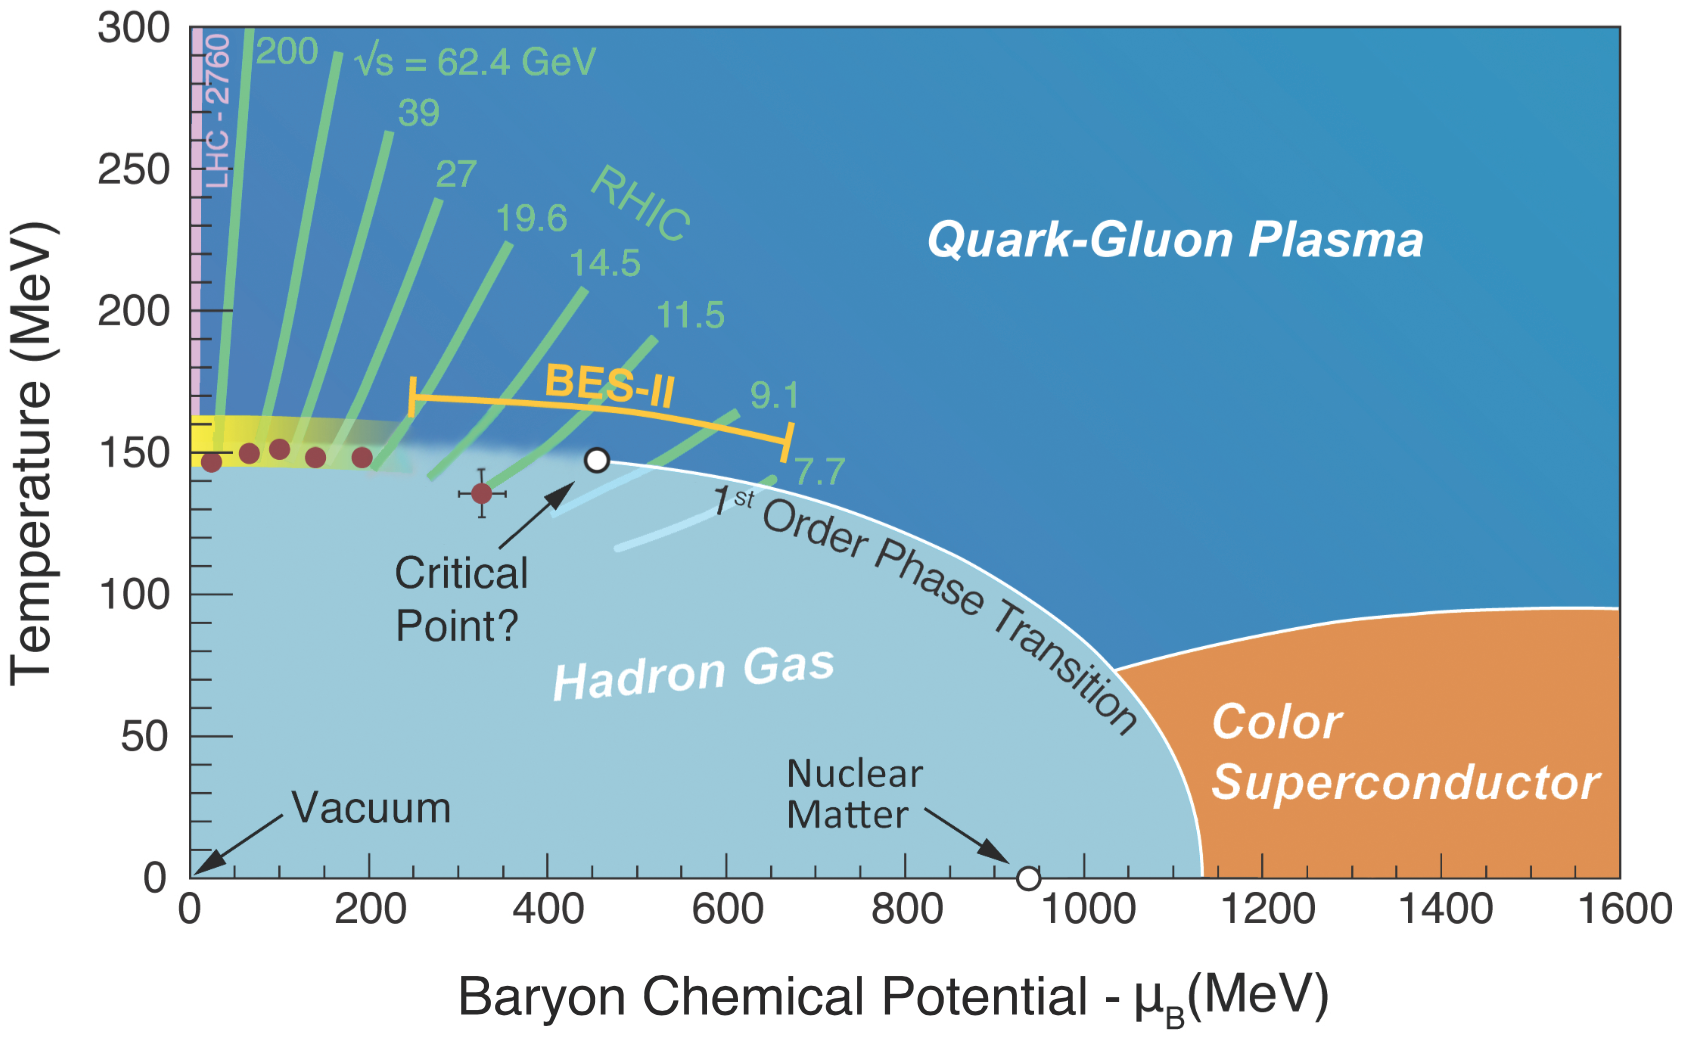
\includegraphics[width=.8\textwidth]{phase-diagram.png}
    \caption{The (partly projected) phase-diagram of the nuclear matter from reference []. The horizontal variable is Baryon chemical potentail $\mu_B$ and the vertical variable is temperature $T$. The red and green trajectories indicates the reachable regions by the heavy-ion program at the LHC and RHIC.}
    \label{fig:phase-diagram}
\end{figure}

Moving to wards finite baryon chemical potential, the lattice approach runs into the fermion sign problem, though recent studies has been pushing the realm of lattice QCD into small $\mu/T$ regions \cite{Gunther:2016vcp,Bazavov:2017dus}.
Effective models [] and Dyson-Schwinger equation studies [] have suggested the existence of a first order phase transition at large $\mu_B/T$.
If true, the first-order coexistence line must end at a point on the phase-diagram at lower $\mu_b$, beyond which the phase-transition is the cross-over type.
Such a point, called the critical end point (CEP), has attached a great interest of both theoretical confirmation / exclusion and experimental search.

At higher chemical potential and low temperature, another phase of nuclear matter known as the ``color superconducting phase'' is proposed, where the quarks forms Cooper pairs in analogy to the superconductors [].

\begin{figure}
    \centering
    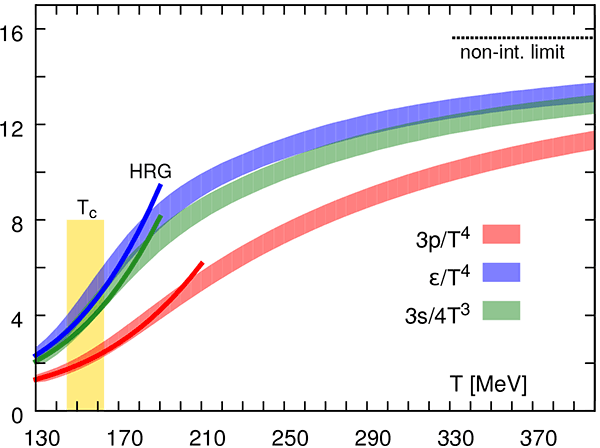
\includegraphics[width=.8\textwidth]{qcd-eos.png}
    \caption{The lattice equation of state for 2+1 flavor QCD taken from reference \cite{Bazavov:2014pvz}. The rescaled pressure, energy density and entropy density as function of temperature at zero chemical potential are shown as red, blue and green bands. The dashed lines indicates non-interaction (Stephan-Boltzmann) limit and the solid lines show the expected values from a hadron resonance gas. The yellow band is the region of pseudo-critical temperature.}
    \label{fig:qcd_eos}
\end{figure}

It is believed that the QCD high-temperature phase-transition is a stage of the universe around a microsecond after ``the Big Bang'', when the temperature drops down to QCD scale.
Compact starts are ``celestial laboratories'' to test the QCD equation-of-state in the high density and low temperature region, providing an important physical input for simulating the recently discovered gravitational wave from neutron star mergers.
In laboratories, we create hot and dense nuclear matter by colliding heavy nuclei at ultra-relativistic high energies.
Though the created matter is so transient and tiny compared to the cosmic nuclear matter, we can learn not only thermodynamic properties but also essential dynamical properties of the QCD in these experiments.

\section{Phenomenology of relativistic heavy-ion collision}
Relativistic heavy-ion collision is currently the only tool to access high energy density QCD medium in laboratory.
Since 2005, the Relativistic Heavy-ion Collider (RHIC) at the Brookheaven National Laboratory (BNL) started colliding gold nuclei at 200 GeV []. 
The Large Hadron Collider (LHC) started its heavy ion programs later, colliding lead nuclei at 2.76 TeV and 5.02 TeV [].
Since then, many evidences have been pointing to the existence a new state-of-matter: the strongly coupled quark-gluon plasma (sQGP).

In this section, I shall introduce useful concepts and terminology in heavy-ion collisions.
Then I will review a few important experimental evidences and how they can help the understanding of the properties of the sQGP.

\subsection{Kinematics}
In ultra relativistic collisions, it is advantages to use a new set of coordinates, related to the Cartesian coordinates by,
\begin{eqnarray}
x_\perp &=& x_\perp\\
\tau &=& \sqrt{t^2 - z^2}\\
\eta_s &=& \frac{1}{2}\ln\frac{t+z}{t-z}
\end{eqnarray}
where the $z$ direction aligns with the accelerated beam direction.
$\tau$ is called the ``proper time" and $\eta_s$ called the space-time rapidity.
One advantage of using this set of coordinates is that $\tau$ and $\eta_s$ transforms much simpler than $t$ and $z$ under Lorentz boost ($\beta_z$) in the beam direction,
\begin{eqnarray}
\tau' &=& \tau,\\
\eta_s' &=& \eta_s + \frac{1}{2}\ln\frac{1+\beta_z}{1-\beta_z}
\end{eqnarray}
Similarly for the four momentum $p^\mu$ is parametrized as 
\begin{eqnarray}
p_x &=& p_T\cos\phi\\
p_y &=& p_T\sin\phi\\
m_T &=& \sqrt{m^2 + p_T^2}\\
y &=& \frac{1}{2}\ln\frac{E+p_z}{E-p_z}.
\end{eqnarray}
$p_T$ is transverse momentum relative to the beam ($z$) direction, $\phi$ is the azimuth angle of particle emission. 
$m_T$ is referred as the transverse mass, and $y$ is the rapidity of a particle.
Besides, pseudorapidity is often used in experiments,
\begin{equation}
\eta = \frac{1}{2}\ln\frac{|p|+p_z}{|p|-p_z} = \frac{1}{2}\ln\frac{1+\cos\theta}{1-\cos\theta}
\end{equation}
It has the merits that it is directly related to the polar angle  $\theta$ of particle emission.
When the transverse mass is small compared to $p_z$, the pseudorapidity is also a good proxy of rapidity.

\subsection{Nuclear collision geometry}
Nuclei are extended objects.
The radius of heavy nuclei approximately scales like $A^{1/3}$ fm, where  $A$ is the atomic number; therefore, the collision geometry plays far more important role than it is in the proton-proton collision.
In the center-of-mass frame,  nuclei ``shrink" in the $z$ direction by the factor $\gamma = (1-v^2)^{-1/2} = E/M$ because of the Lorentz contraction.
$\gamma$ is over $100$ for gold nuclei at top RHIC energy and is more than $2500$ for lead nuclei at the LHC.
As a result, the approaching nuclei takes a short time to penetrating each other $t_L = 2R/\gamma$, while dynamics in the transverse direction can only propagate within a causal circle of $r < t_L$ that is much smaller than the nuclear extend.

\paragraph{Impact-parameter and centrality} Defining the impact parameter $\vec{b}$ as the transverse separation between the center-of-mass of the two approach nuclei,
the initial deposition of the energy largely depends on $\vec{b}$.
The collision geometry is a useful handle to study QGP dynamics; however,
it is impossible control $b$ directly in high energy experiments.
What is used as an approximate geometry indicator is the so-called centrality.
Centrality are defined in different ways (detector response / multiplicity / transverse energy) and with different kinematic cuts, but the idea that  nuclear collision geometry strongly correlates with the particle production activity.
It is reasonable to anticipate that the average number of charged particles produced or the total transverse energy deposited within a certain detector's acceptance is higher if the collision is more central (small impact parameter), and is lower for peripheral collision (large impact parameter).
Of course the relation between centrality and impact-parameter is not exact, as dynamical fluctuations smear out the one-to-one correspondence between the impact parameter and the ``centrality meter''.
Correctly accounting for these fluctuations is particularly important for small collision system,s such as proton-lead and deutron-gold collisions.

\paragraph{Centrality selection} Experimentally, a minimum-biased (a minimum set of event triggers) sample of recorded events are sorted according to the centrality definition (multiplicity, e.g.) and the events are binned by percentile.
Then, for example, the top 0--5\% highest multiplicity events are associated to the central collisions with centrality range 0--5\%. 
And the details of the collision geometry can be studied through a model.
Usually, the models is one of the many variants of the Glauber model \cite{Miller:2007ri}, we shall explained it in detail in section \ref{simulation}).
It computes the number of binary nucleon-nucleon ($N_{\textrm{bin}}$) collisions and number of participant nucleons ($N_{\textrm{part}}$, nucleons that suffers at least one binary collisions) at a given impact parameter.
Experimentally, $N_{\textrm{part}}$ is often used as the centrality estimator of the model as it is roughly proportional to the bulk particle production; while the cross-section of hard processes that involves large momentum transfer $Q \gg \Lambda$ scales like the $N_{\textrm{bin}}$.
Though this correspondence can be model dependent, but the uncertainty can be quantified and its prediction can be validated by the production of colorless probes.

\subsection{Particle production at low-$p_T$ and collective flow} 
Immediately after the nuclei penetration through each other $t\sim 2R/\gamma$, huge amount of energy is deposited into the overlapped area and entropy is produced, creating a fireball in the middle while the nuclear remnants recede.
This highly excited fireball of fields undergoes complex dynamics and cools down rapidly because of the longitudinal and transverse expansion.
Eventually, the system hardronizes, and the hadrons can have further interactions and may decay into other hadrons, photons and lepton that are seen by the detectors.

It is observed that the particle production in relativistic nuclear collisions distributes across a wide (pseudo)rapidity range, and has steep falling transverse momentum spectra [].
The majority of the particles are soft hadrons with relatively small transverse momentum $p_T \lesssim 3$ GeV and their creation are consequences of final state interactions [].
One of the most striking discoveries from RHIC and LHC heavy-ion program is that these soft particles displays a strong collectivity and the patterns can be described by viscous hydrodynamic-based models to a very high precision \cite{Dusling:2007gi,Song:2008si,Schenke:2010nt,Petersen:2008dd,Niemi:2015qia,Bernhard:2016tnd,Bernhard:2018hnz}.
This success of the hydrodynamic model reveals the strongly coupled nature of the matter produced with a temperature several times above $T_c$ and it has been entitled the name strongly coupled quark-gluon plasma.
This is in contrary to a weakly coupled gas of quarks and gluons that emits independently.

\begin{figure}
\centering
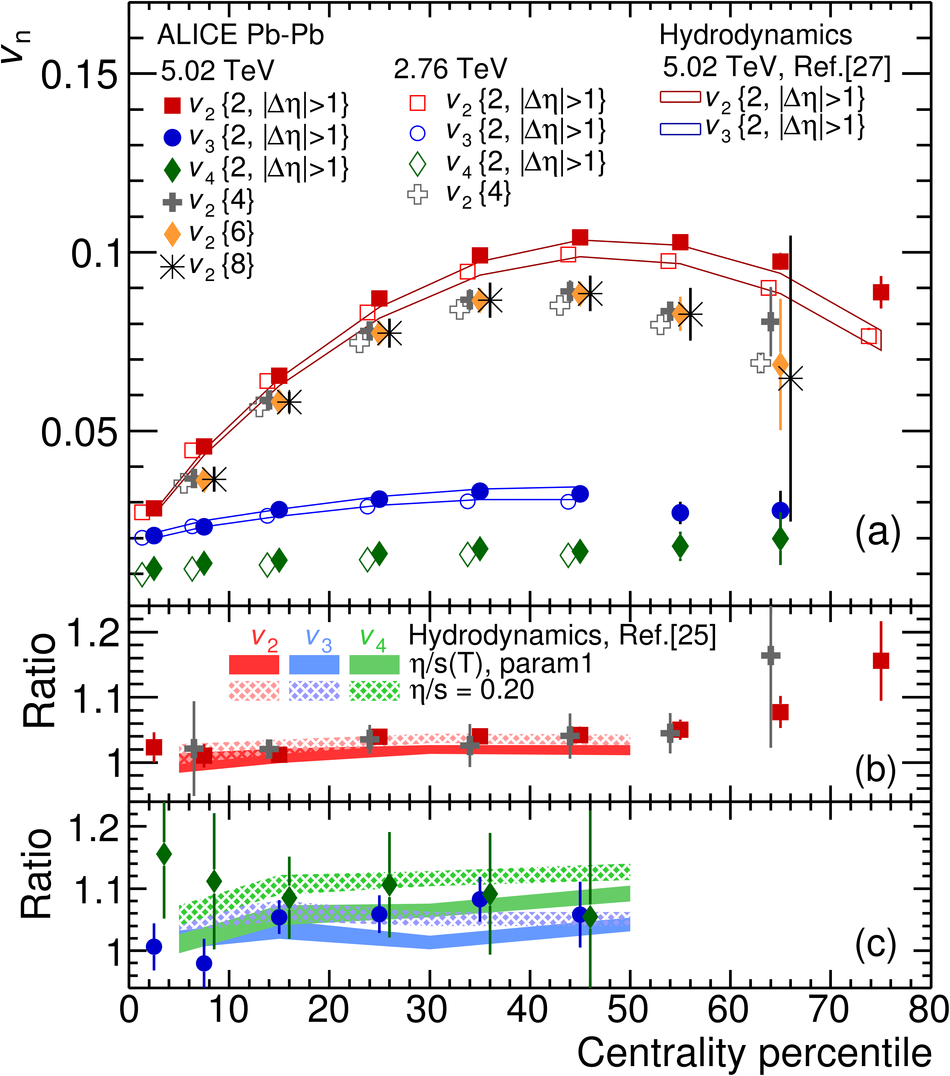
\includegraphics[width=.6\textwidth]{ALICE-chg-vn.png}
\caption{The momentum anisotropy coefficient $v_2$ estimated from multi-particle correlation for charged particle from the ALICE collaboration [].
The hydrodynamic-based calculations [] (lines) very well explains the centrality dependence of the second (red), third (blue) and fourth (green) order coefficients at different beam energies.}
\label{fig:intro:vn}
\end{figure}

One manifestation of collectivity is the momentum space anisotropy or collective flow of the bulk medium.
Decompose the charged particle spectra into Fourier series of the azimuth angle,
\begin{eqnarray}
E\frac{dN}{p_T dp_T d\phi dy} = \frac{1}{2\pi}\frac{dN}{p_T dp_T dy}\left(1 + 2\sum_{n=1}^{\infty}v_n(p_T)\cos\left[n(\phi-\Psi_n)\right]\right).
\end{eqnarray}
The first term is averaged yield, and subsequent terms in the sum encode the angular dependence. 
The $n=1$ term is a shift of the center-of-mass momentum
From $n=2$, $v_n$s are momentum anisotropy coefficients of $\cos({n\phi})$ modulations.
If the particle production is simply an independent sum of elementary nucleon binary collisions, then the anisotropy would be zero after average. 
However, experiments observe a surprisingly larger elliptic flow ($v_2$), triangular flow ($v_3$) and higher order $v_n$ at both RHIC and LHC in nuclear collisions.
Figure \ref{fig:intro:vn} shows the variation of the $v_n$ as function of centrality from ALICE measurements [].
The $v_2$ coefficients first increases from central to mid-central collisions and slightly decreases at peripheral collisions, while $v_3$, $v_4$ signal are smaller and varies slower with centrality.

In the hydrodynamic picture, a non-central collision deposits initial energy density in an almond shape and the initial fireball has a finite spatial eccentricity $\epsilon_2$.
The energy density is higher in the middle and lower at the boundary, so a hydrodynamic pressure builds up and drives the transverse expansion of the fireball.
Because the pressure gradient is larger in the short axis-direction and the long-axis direction, the matter flows in an isotropic way, creating the observed momentum space second-order anisotropy $v_2$.
The existence of higher order of flow harmonics and non-zero $v_2$ in the most central collisions is because the nuclear configuration fluctuations, such as randomized nucleon positions, create all order of eccentricity $\epsilon_n$.
In short, a hydrodynamic expansion transfer initial geometry eccentricities $\epsilon_n$ into final state momentum anisotropy $v_n$ of the particle.

\paragraph{Extracting the QGP transport coefficients}
A relativistic ideal hydrodynamic model assumes an infinitely strong interaction that the medium always stages in local thermal equilibrium.
A more sophisticated treatment is the relativistic viscous hydrodynamics to account for deviations from the local thermal equilibrium due to large gradients in the expansion.
The response of hydrodynamic evolution to the gradients are characterized by the shear viscosity $\eta$ and bulk viscosity $\zeta$.
The QGP shear viscosity and bulk viscosity are of fundamental importance. 
The shear viscosity to entropy ratio $\eta/s$ is an indicator of the stong / weak coupling nature of the QGP. 
And the bulk viscosity to entropy ratio $\zeta/s$ is directly related to  the scale-invariance breaking of QCD.

Dynamical quantities such as viscosity are extremely hard to be computed from first principle, so currently, the pinning down of these numbers and their temperature dependence resorts to the phenomenological extraction from experiments \cite{Muronga:2004sf, Chaudhuri:2006jd, Romatschke:2007mq, Dusling:2007gi, Song:2007ux, Luzum:2008cw}.
The flow harmonics $v_n$ are particular sensitive to the viscous effects, as a finite viscosity damps the development of anisotropic flows, reducine the transition efficiency from $\epsilon_n$ to $v_n$.
Global comparisons of the state-of-the-art medium modeling to a collection of soft observables have corroborated the need of a small $\eta/s$ that are likely to be slowly increasing with temperature and a non-vanishing $\zeta/s$.

\subsection{Probing sQGP using hard probes}
Very occasionally, an initial collision involves large momentum transfer creates high-$p_T$ particles in the system ($p_T\gtrsim 10$ GeV), are referred to as the ``hard" particles.
By uncertainty principal, they can only be produced at the beginning of the nuclear collision on a time scale $\delta t \sim 1/p_T$, then they pass through and interact with the surrounding bulk medium.
Hard particles can be used as self-generated probes of the system.
Due the asymptotic freedom, the initial production of hard processes can be computed in the perturbative framework, granting a good theoretical control of its initial state.
The final state interaction with the medium then modifies the initial production and leaves finger prints of the medium on the hard probes.

\paragraph{Jet and jet quenching}
Initial hard partons (gluons, quarks) undergoes complex QCD dynamics, radiating more partons which then hadronizes into a collimated bunch of hadrons and decay products.
This final collection of particles is observed in detector as jets.
In the proton-proton collisions, perturbative calculations and Monte-Carlo simulations are able to explains the production cross-section of the jet and leading hadrons (the hardest hadron in the jet) reasonably well.
In the nuclear collisions, the initial parton and the radiative daugther partons interacts with the medium, causing energy loss and triggering medium-induced radiation.
As a result, one expects the jet / leading parton yield at high-$p_T$ is reduced compared to the reference in proton-proton.
To focus on the difference caused by medium effects, the reference has to cancel out a na\"ive difference that simply rises because there are more effective nucleon-nucleon collisions than the proton-proton collisions.
One defines the so-called ``nuclear modification factor'',
\begin{eqnarray}
R_{AA}(y, p_T) = \frac{\frac{dN_{AA}}{dy dp_T}}{\langle N_{\textrm{coll}}\rangle \frac{dN_{pp}}{dy dp_T}} = \frac{\frac{dN_{AA}}{dy dp_T}}{\langle T_{AA} \rangle \frac{d\sigma_{pp}}{dy dp_T}}.
\end{eqnarray}
It is the average $N_{\textrm{bin}}$ ``normalized'' ratio between the yield in AA collisions and pp collision.
The number of binary collision is sometimes replaced by the average nuclear overlapping function $\langle N_{\textrm{coll}}\rangle = \langle T_{AA} \rangle /\sigma_{pp}^{\textrm{inel}}$, and the yield is replaced by the inclusive cross-section for the proton-proton collision $\frac{dN_{pp}}{dy dp_T}\rightarrow \frac{d\sigma_{pp}}{dy dp_T}$.
These two expressions are equivalent.
The ratio is expected to be unity if there is no medium effect, though we do remind the readers that $N_{\textrm{coll}}$ is not a directly observed quantity and has to be estimated in a model-dependent way.

At both RHIC and the LHC, colored probes as measured by the $R_{AA}$ of leading hadron and jet are found to be significantly below unity in nuclear collisions, while  $R_{AA}$ of color neutral probe such as $Z$-boson is consistent with unity.
These discoveries indicate the creation of a color deconfined medium that strongly modifies to hard parton propagation.
The interaction strength between the hard parton and the medium is theoretically quantified as the jet transport parameter $\hat{q}$, which is defined as the momentum broadening per unit path-length in the transverse direction of the propagation,
\begin{eqnarray}
\frac{d\langle p_\perp^2 \rangle}{dL} = \hat{q}
\end{eqnarray}
The jet transport coefficients is another quantity of fundamental interest  in heavy-ion collisions, and there has been a great effort in both first principal computation and phenomenological extraction \cite{Wang:1994fx,Zakharov:1996fv,Baier:1996sk,Zakharov:1997uu,Arnold:2002zm,Gyulassy:2003mc,Kovner:2003zj,Jeon:2003gi,CasalderreySolana:2007pr,Djordjevic:2008iz,Bass:2008rv,Schenke:2009gb,Majumder:2009zu,Majumder:2010qh,Armesto:2011ht,Zapp:2011ya,Ovanesyan:2011xy,Kang:2014xsa,Cao:2016gvr,Kauder:2018cdt,Cao:2017zih}.
The hard parton / jet probes the medium at different scale at different stage of its evolution, and more sophisticated observables and theoretical tools are being constructed to answer more microscopic questions such as the actually degrees of freedom of the strongly coupled QGP.
Future experimental upgrades might provide the precisions to look into this problems \cite{ATLAS-Collaboration:2012iwa,Abelevetal:2014dna,STAR:upgrade-hf,Adare:2015kwa,CMS:2017dec}.

\paragraph{Heavy-flavor probes}
Heavy flavor is a charming probe in studying heavy-ion collisions, and is also the focus of this work.
Heavy quarks have mass well above the QCD non-perturbative scale.
The charm quark ($M=1.3$ GeV) and bottom quark (M=$4.2$ GeV) are the most relevant heavy quarks for the present study.
The reason that top quark ($M = 173$ GeV) is out of our discussion is due to its extremely short life time ($\sim 5\times 10^{-25} \approx 0.15$  fm/$c$ in its rest frame) so it barely interacts with the QGP before it decays into, predominantly, bottom quarks.
Though there has also been proposal that takes the advantage of this short life-time to probe the temporal structure of the QGP evolution, we only focus on the charm and bottom flavor in this work.

\begin{figure}
\centering
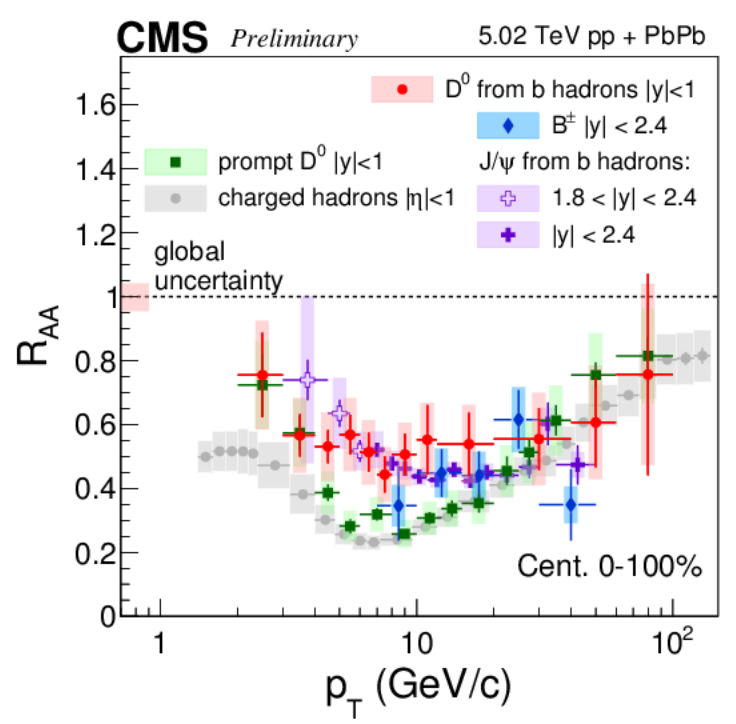
\includegraphics[width=.7\textwidth]{CMS-HF.png}
\caption{The nuclear modification factor $R_{AA}(p_T)$ of charged hadron (gray), D meson (red), B meson (blue), and $b$-decayed D meson (red), $b$-decayed J$/\Psi$ (purple) measured by the CMS collaboration [].}
\label{fig:intro:Raa}
\end{figure}

A large mass guarantees a negligible thermal production contribution, at least for the present top LHC beam energies (there are estimations that thermal contribution can play a row in future FCC collider []).
Therefore, heavy flavors, regardless of its $p_T$, are almost always created in initial hard processes.
Moreover, the tiny population of heavy flavors in the collision also suppresses the chances that they annihilates / recombine with their anti-particles.
Certainty heavy mesons have a long life time such that the decay vertices are outside of the fireball and can be resolved by experiments.
Therefore, the number of heavy-flavor particles is almost conserved from the beginning to the end of the entire medium evolution including both the QGP phase and the hadronic phase.

\begin{figure}
\centering
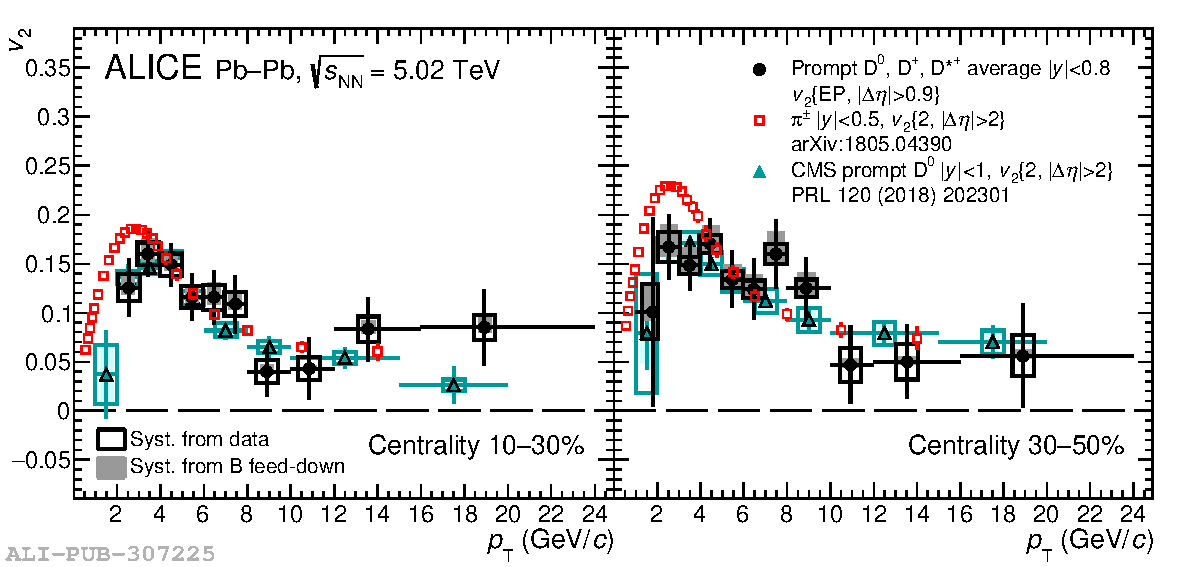
\includegraphics[width=\textwidth]{ALICE-CMS-D-vn.pdf}
\caption{The charged pion (red) and D meson momentum anisotropy measured by the ALICE Collaboration (black) and the CMS Collaboration (green). Left and right panels show the results for 10-30\% centrality and 30-50\% centrality respectively.}
\label{fig:intro:D-vn}
\end{figure}

Heavy flavors are of physical interests in many ways.
The mass effects are negligible at high $p_T$ where heavy flavors merge into the topic of the jet energy loss physics.
At intermediate $p_T$, the mass effect is expected to suppress the medium-induce radiation, which dominates the energy loss of light quark.
And there may be a competing between the collisional energy loss and radiation processes.
Experimentally, these differences lead to a hierarchy in the amount of nuclear suppression.
For example, figure \ref{fig:intro:Raa} citing from the CMS collaboration shows a collection of $R_{AA}$ measurements, for charged (mostly light) hadron, prompt D meson, prompt B meson and D and J/$\Psi$ from $b$-decays.
All the $R_{AA}$ tends to collapse onto the same trend at very high-$p_T$, while for $p_T$ range aounrd 5 to 20 GeV, despite the large uncertainty, there is a suggestive hierarchy of $R_{AA}(\textrm{light}) < R_{AA}(\textrm{charm}) < R_{AA}(\textrm{bottom})$.
It would be interesting to study whether the theoretical framework can explain this difference quantitatively and distinguish different energy loss mechanisms.

Low-$p_T$ heavy quark physics is even more interesting.
In this region, collisional process dominates over radiative process, and the description of the heavy quark dynamics under the influence of medium ``kicks'' reduces to the succinct diffusion equation \cite{Moore:2004tg}.
A spatial diffusion constant $D_s$ controls the close-to-equilibrium dynamics, and canbe related to the momentum diffusion by $D_s = 4T^2/\hat{q}(p\rightarrow 0)$ [].
The large inertia $M\gg T$ delays its relaxation time $\tau_{\textrm{th}} \propto M/T D_s$ and one expects to find a different degree of thermalization for light, charmed, and bottom hadrons \cite{PhysRevD.37.2484,Moore:2004tg,Riek:2010fk,Cao:2013ita}.
For instance, looking at the low $p_T$ momentum anisotropy of charmed meson shown in figure \ref{fig:intro:D-vn} \cite{Acharya:2017qps,Sirunyan:2017plt}.
The large $v_2$ of the charged pions below $3$ GeV is due to the collective expansion.
The charmed mesons also catch up a significant amount of flow \footnote{As a remark, the finite $v_2$ of D meson at high $p_T$ is not directly related to the flow phenomena, but as a result of anisotropic energy loss in a spatial eccentric medium}, though still less than the pion.
To explains this amount of D meson $v_2$, phenomenological studies suggests a $D_s$ close to the lattice QCD evaluations \cite{He:2012df,Cao:2013ita,Xu:2017obm,Banerjee:2011ra,Ding:2012sp,Francis:2015daa}, while leading order weakly coupled result \cite{Moore:2004tg} is inadequate . 
This finding suggests the importance of non-perturbative phenomenon in understanding the coupling between low momentum heavy quark and the medium.

Finally, the unique flavors of heavy quarks help to tag certain processes of interest. 
For example, the study of recombination hadronization mechanism, strange ness enhancement, and implementing a selection bias on the quark / gluon-initiated jet ratio.

\subsection{Transport modeling of hard probes}
The understanding of jets and heavy-flavor in heavy-ion collisions needs a comprehensive non-equilibrium modeling.
This includes initial production / DGLAP evolution, the partonic propagation in the QGP, and eventually the hadronic interaction.
Transport equations are convenient tools to couple the microscopic hard probes propagation to the macroscopic medium evolution, though one have to be very careful with the multiple scales of the problem.
For example DGLAP evolution brings the parton scale from $p_T$ down to O(GeV).
The probe-medium interactions happens at typical scales around temperature $T$ and the screening mass $m_D \sim gT$, while the medium-induced radiation suffers momentum broadening scale of order $\hat{q} t$.
Eventually, hadronization happens at scale $\Lambda$.
Meanwhile, the medium evolution has a another set of (time) scales, the hydrodynamization time $\sim 1$ fm/$c$, the finite-size and life-time of the QGP fireball $\sim O(10)$  fm/$c$, and the expansion time scale $\tau_{\textrm{ex}}$.
Usually a well separation of scales allows great simplification to the theory calculations.
For example, the Boltzmann transport equation requires a separation between the mean-free-path and the coherence time of the scattering.
However, in realistic event simulations, treating regions of overlapping scales seems inevitable.
We would like to develop in this thesis a new transport model to account for a few of these overlapping scale issues.

\paragraph{Heavy quark transport models}
In early days, the heavy quark measurements at RHIC energy does not extend to very high-$p_T$ and the radiative energy loss is not as important as elastic ones.
And one study the non-equilibrium dynamics using a pure diffusion model \cite{Moore:2004tg,vanHees:2007me}. 
To include physics at high-$p_T$ physics, a radiation improved diffusion model was then developed \cite{Cao:2013ita} and has been applied to the first Bayesian extraction of the heavy quark transport coefficients \cite{Xu:2017obm}.
Apart from the diffusion-based models, Boltzmann and linearized Boltzmann models, including both elastic and inelastic interactions, are also developed \cite{Scardina:2017ipo,Cao:2017hhk,Ke:2018tsh}.
Regarding the physical inputs, the Boltzmann-based model takes a weakly-coupled picture; the diffusion based model is more flexible, since the transport coefficient can be computed in both weakly coupled or strongly coupled approaches.
Using different models, the extracted transport parameters $D_s$, $\hat{q}$ have notable differences \cite{Rapp:2018qla,PhysRevC.99.014902,Cao:2018ews}.
The major sources that leads to these differences are:
\begin{itemize}
\item Whether the radiative energy loss is included.
\item Assumptions on the medium: close-to-equilibrium hydrodynamic medium, or non-equilibirum form full partonic Boltzmann equation.
\item Weakly coupled approach versus strongly coupled approach.
\item More subtle differences such as Langevin versus Boltzmann dynamics, and the detailed treatment of the radiative process.
\end{itemize}
To make convergent progress, on the one hand improved theoretical calculations and more accurate modeling is important; on the other hand, more subtle differences should can be treated as intrinsic modeling uncertainty so that the extracted transport parameters are not over-interpreted (a finite theoretical uncertainty bands on $D_s$ and $\hat{q}$). 
I will also try to make progress in this direction.

\subsection{Understanding QGP as a parameter inference problem}
All the interesting dynamics of heavy-ion collision only last for $O(10) $ fm/$c$, while we can only observe the collision remnants by detectors meters away.
Therefore, the learning of any intrinsic properties of QGP is essentially  a parameter inference problem:
given measurements, models, and parameters of QGP such as $\eta/s, \hat{q}$, what is the favored range of parameters to explain the data.
Finally, by comparing the theoretical expectations (if exists) and the phenomenological constraints of these parameters, one evaluate the theoretical assumptions, which gives out new information of the QGP.

This inversion from observables to parameters is not as simple as it appears, because of the following difficulties,
\begin{itemize}
\item The dynamical models are complex and computationally intense.
\item Model takes multiple parameters or unknown functions that have infinitely many degrees of freedom.
\item Global comparison to many experimental observables.
\item The quantification of uncertainty: including experimental uncertainty, model uncertainty and theoretical uncertainty.
\end{itemize}
Most of these issues can be solved by the Bayes analysis for model parameter calibration, and its key ingredients will be explained in chapter \ref{chapter:bayes}.
A remaining issue is the theoretical uncertainties, which is hard to quantify.
Our solution to the theoretical uncertainty is two-folded.
First, if there are more than one theoretical assumptions without appealing reasons to disfavor either of them, then this difference should be propagated into the extracted model parameters.
Including these uncertainty will certainly decrease the constraining power on the transport parameters, but it prevents biasing the estimated number from imposing a too strong assumption.
Second, existing theoretical calculations are often worked out in certain idealized limits, while a dynamical modeling is much more complicated and may not closely follow what the underlying theory.
This will certainly obscure the interpretation of the extracted parameters.
Therefore, as an important practice for dynamical modeling, the model should be able to calibrate to theoretical calculations at least in those idealized limits, and then generalized to the more complex scenario.
We devoted chapter \ref{transport} to improve the accuracy of hard parton transport model.

\section{Outline of this Thesis}
In this thesis, I focuses on the extraction of the heavy quark transport coefficients from experiments using a newly developed transport model for hard parton in a quark-gluon plasma.
In chapter \ref{chapter:simulation}, I introduce a hydrodynamic-based medium for the medium evolution. 
As an application of this simulation framework, I review my project on reverse engineering a three-dimensional initial entropy deposition of the heavy-ion collision from experimental data. 
In chapter \ref{chapter:transport}, we develop the transport model for hard partons (including heavy flavors) propagation inside a quark-gluon plasma.
This model interpolates a small-angle diffusion picture and a large-angel scattering picture of the probe-medium interaction.
I show the limitation of the semi-classical transport approach in implementing parton branching processes (radiation) at high energy, and demonstrate how to modified the semi-classical approach to treat it properly.
Chapter \ref{chapter:coupling} builds a comprehensive simulation workflow that couples the initial production and in-meidum transport of heavy flavors to the bulk medium evolution.
Benchmark calculations with simple guesses of parameters are compared to the experimental measurements.
Chapter \ref{chapter:bayes} is a brief description of the Bayes methodology of model parameter calibration.
Applying the Bayes method, in chapter \ref{chapter:results}, a systematic model-to-data comparison is performed, extracting the heavy flavor transport properties.
Finally, chapter \ref{chapter:conclusion} summarizes the work and discuss possible future improvements.


